\documentclass[13pt, a4paper, titlepage]{report}
\usepackage[utf8]{vietnam}
\usepackage{amsmath}
\usepackage{amsfonts}
\usepackage{amssymb}
\usepackage[cc]{titlepic}
\usepackage{graphics}
\usepackage[dvipdfmx]{graphicx}
\usepackage{caption}
\usepackage{booktabs}
\usepackage{float}
\usepackage{hyperref}
\usepackage{tkz-tab}
\usepackage{enumitem}

%%%
\begin{document}
\title{BÀI THI CUỐI KÌ \\
		MÔN PHẦN MỀM TOÁN NĂM 2021 \\[4ex]
		
\includegraphics[width=4cm]{images/cover/dhsp_logo.png}}
\author{Họ tên: Nguyễn Thị Hương} 
\date{Ngày nộp bài: \today \\
\ \\
Giáo viên hướng dẫn: Nguyễn Đức Mạnh}
\maketitle

%%%
%\section*{Bài 1:}
Cho 4 điểm $A, B, C, D$ không cùng thuộc một mặt phẳng. Trên các đoạn thằng $AB, AC, BD$ lần lượt lấy các điểm $M, N, P$ sao cho $MN$ không song song với $BC$. Tìm giao tuyến của $(BCD)$ và $(MNP)$.
\begin{figure}[H]
\centering
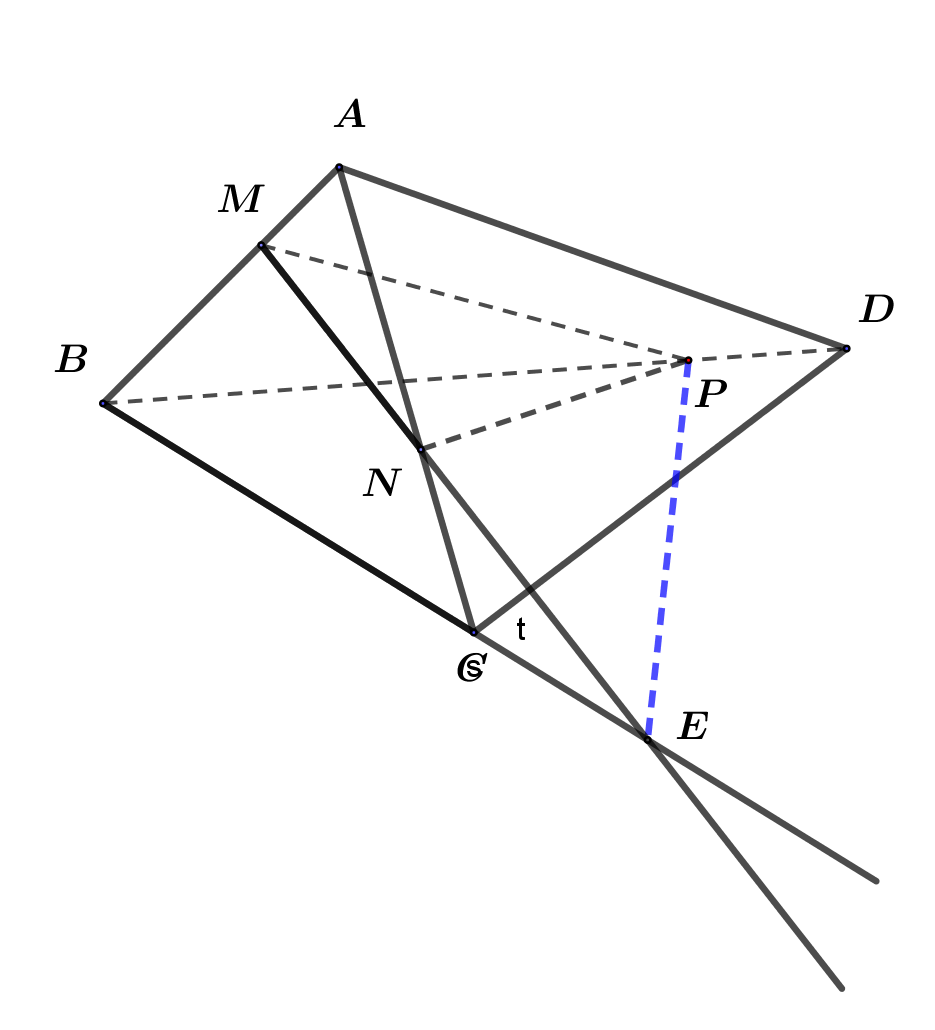
\includegraphics[width=6cm]{images/quizz1/quizz_1_figure.png}
\caption{Hình vẽ bài 1}
\end{figure}

\subsection*{Lời giải:}
\begin{itemize}
\item Ta có $P \in BD$ mà $BD \subset (BCD) \Rightarrow P \in (BCD)$ 
\item Mặt khác ta lại có $ P \in (MNP) $
\end{itemize}
$\Rightarrow P$ là điểm chung của $(BCD)$ và $(MNP)$

\vspace{5mm}
Trong mặt phẳng $(ABC)$ gọi $E = MN \cap BC$
\begin{itemize}
\item $ E \in BC$ mà $BC \subset (BCD) \Rightarrow E \in (BCD)$
\item $ E \in MN$ mà $MN \subset (MNP) \Rightarrow E \in (MNP)$
\end{itemize}
$\Rightarrow E$ là điểm chung của $(BCD)$ và $(MNP)$

\vspace{5mm}
Từ trên ta suy ra kết luận:
$PE$ là giao tuyến của 2 mặt phẳng $(BCD)$ và $(MNP)$
\section*{Bài 1:}
Cho 4 điểm $A, B, C, D$ không cùng thuộc một mặt phẳng. Trên các đoạn thằng $AB, AC, BD$ lần lượt lấy các điểm $M, N, P$ sao cho $MN$ không song song với $BC$. Tìm giao tuyến của $(BCD)$ và $(MNP)$.
\begin{figure}[H]
\centering
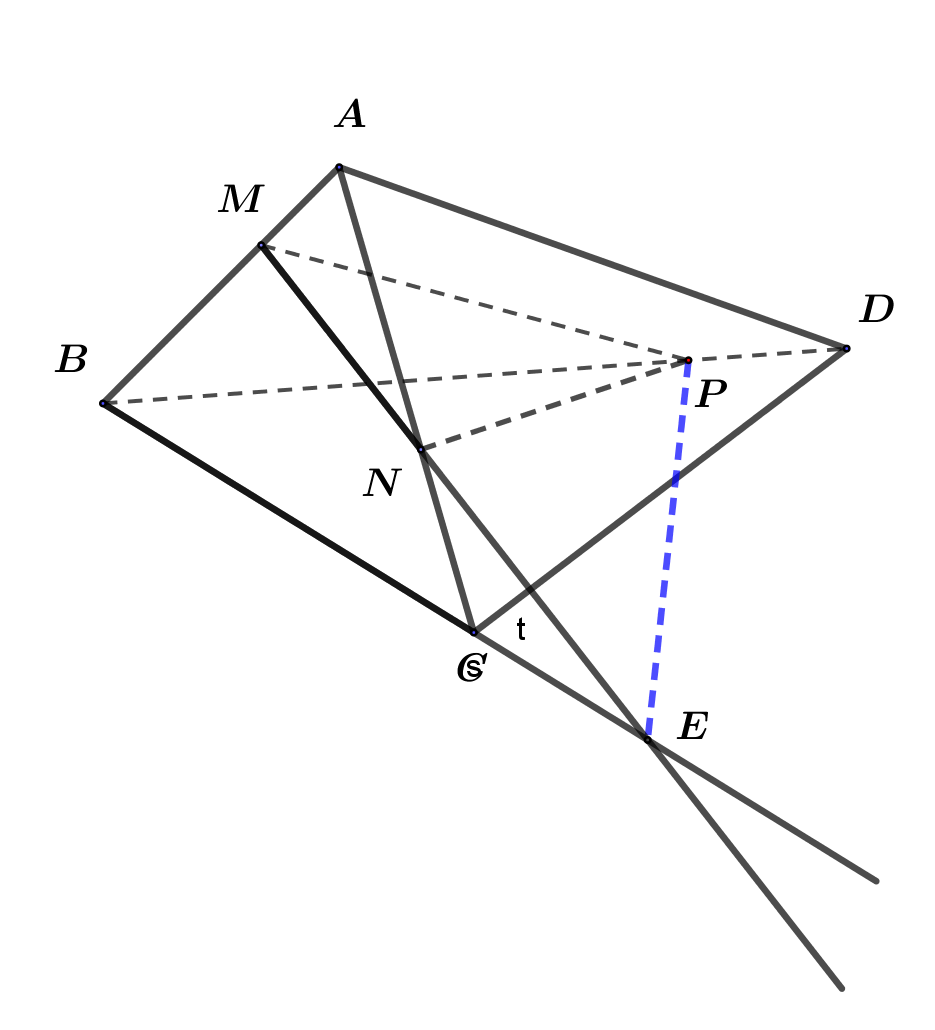
\includegraphics[width=6cm]{images/quizz1/quizz_1_figure.png}
\caption{Hình vẽ bài 1}
\end{figure}

\subsection*{Lời giải:}
\begin{itemize}
\item Ta có $P \in BD$ mà $BD \subset (BCD) \Rightarrow P \in (BCD)$ 
\item Mặt khác ta lại có $ P \in (MNP) $
\end{itemize}
$\Rightarrow P$ là điểm chung của $(BCD)$ và $(MNP)$

\vspace{5mm}
Trong mặt phẳng $(ABC)$ gọi $E = MN \cap BC$
\begin{itemize}
\item $ E \in BC$ mà $BC \subset (BCD) \Rightarrow E \in (BCD)$
\item $ E \in MN$ mà $MN \subset (MNP) \Rightarrow E \in (MNP)$
\end{itemize}
$\Rightarrow E$ là điểm chung của $(BCD)$ và $(MNP)$

\vspace{5mm}
Từ trên ta suy ra kết luận:
$PE$ là giao tuyến của 2 mặt phẳng $(BCD)$ và $(MNP)$

%\section*{Bài 2:}
Khảo sát sự biến thiên và vẽ đồ thị hàm số: $y = -x^3 + 3x^2 - 4$

\subsection*{Lời giải:}
\begin{itemize}
\item[$\ast$] Tập xác định D=R
\item[$\ast$] Chiều biến thiên:
Ta có: $y^{\prime} = -3x^2 + 6x = -3x(x-2)$ \\
Xét phương trình $y^{\prime} = 0 \Leftrightarrow -3x(x-2) = 0 \Leftrightarrow x = 0$ hoặc $x = 2$
\item[$\ast$] Bảng biến thiên:
	\begin{figure}[H]
		\centering
		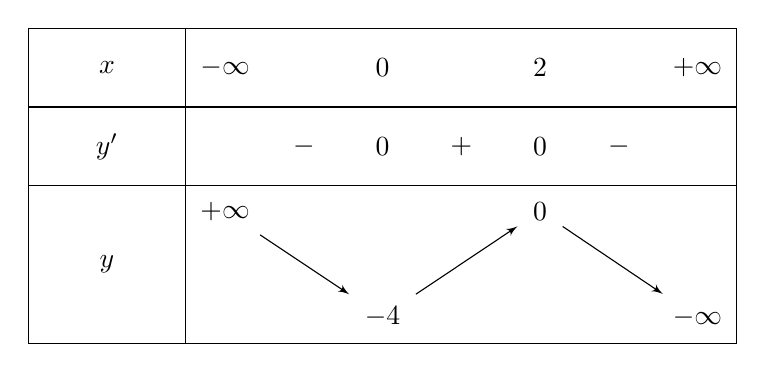
\begin{tikzpicture}
			\tkzTabInit[nocadre=false,lgt=2,espcl=2]
			{$x$ /1,$y'$ /1,$y$ /2}
			{$-\infty$,$0$,$2$,$+\infty$}
			\tkzTabLine{,-,$0$,+,$0$,-,}
			\tkzTabVar{+/ $+\infty$ ,-/$-4$,+/$0$,-/$-\infty$}
		\end{tikzpicture}
	\end{figure}
	Hàm số nghịch biến trên các khoảng $(-\infty; 0)$ và $(2; +\infty)$, đồng biến trên khoảng $(0; 2)$ \\
	Hàm số đạt cực đại tại điểm $x=2$, giá trị cực đại của hảm số là $y(2)=0$. \\
	Hàm số đạt cực tiểu tại điểm $=0$, giá trị cực tiểu của hàm số là $y(0)=-4$ \\
	Giới hạn của hàm số tại vô cực: 
	$$\lim_{x \to -\infty}{y} = +\infty$$
	$$\lim_{x \to +\infty}{y} = -\infty$$
\item Đồ thị:
	\begin{figure}[H]
		\centering
		
\includegraphics[width=6cm]{images/cover/dhsp_logo.png}
		\caption{Hình vẽ đồ thị bài 2}
	\end{figure}
	Cho $x = 1 \Rightarrow y = 0$ \\
	Cho $x = 3 \Rightarrow y = -4$
\item Điểm uốn:
	$$y^{\prime\prime} = -6x + 6 = 0 \Leftrightarrow x = 1$$
	Khi $x = 1 \Rightarrow y(-1) = 2$ \\
	Đồ thị hàm số nhận điểm $I(-1, 2)$ làm điểm uốn. 
\end{itemize}


\section*{Bài 2:}
Khảo sát sự biến thiên và vẽ đồ thị hàm số: $y = -x^3 + 3x^2 - 4$

\subsection*{Lời giải:}
\begin{itemize}
\item[$\ast$] Tập xác định D=R
\item[$\ast$] Chiều biến thiên:
Ta có: $y^{\prime} = -3x^2 + 6x = -3x(x-2)$ \\
Xét phương trình $y^{\prime} = 0 \Leftrightarrow -3x(x-2) = 0 \Leftrightarrow x = 0$ hoặc $x = 2$
\item[$\ast$] Bảng biến thiên:
	\begin{figure}[H]
		\centering
		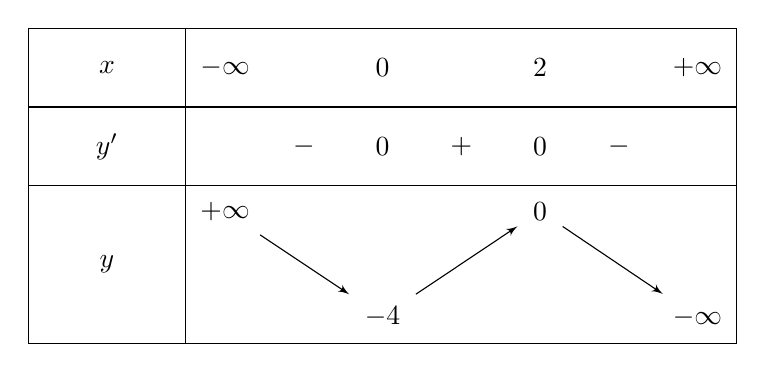
\begin{tikzpicture}
			\tkzTabInit[nocadre=false,lgt=2,espcl=2]
			{$x$ /1,$y'$ /1,$y$ /2}
			{$-\infty$,$0$,$2$,$+\infty$}
			\tkzTabLine{,-,$0$,+,$0$,-,}
			\tkzTabVar{+/ $+\infty$ ,-/$-4$,+/$0$,-/$-\infty$}
		\end{tikzpicture}
	\end{figure}
	Hàm số nghịch biến trên các khoảng $(-\infty; 0)$ và $(2; +\infty)$, đồng biến trên khoảng $(0; 2)$ \\
	Hàm số đạt cực đại tại điểm $x=2$, giá trị cực đại của hảm số là $y(2)=0$. \\
	Hàm số đạt cực tiểu tại điểm $=0$, giá trị cực tiểu của hàm số là $y(0)=-4$ \\
	Giới hạn của hàm số tại vô cực: 
	$$\lim_{x \to -\infty}{y} = +\infty$$
	$$\lim_{x \to +\infty}{y} = -\infty$$
\item Đồ thị:
	\begin{figure}[H]
		\centering
		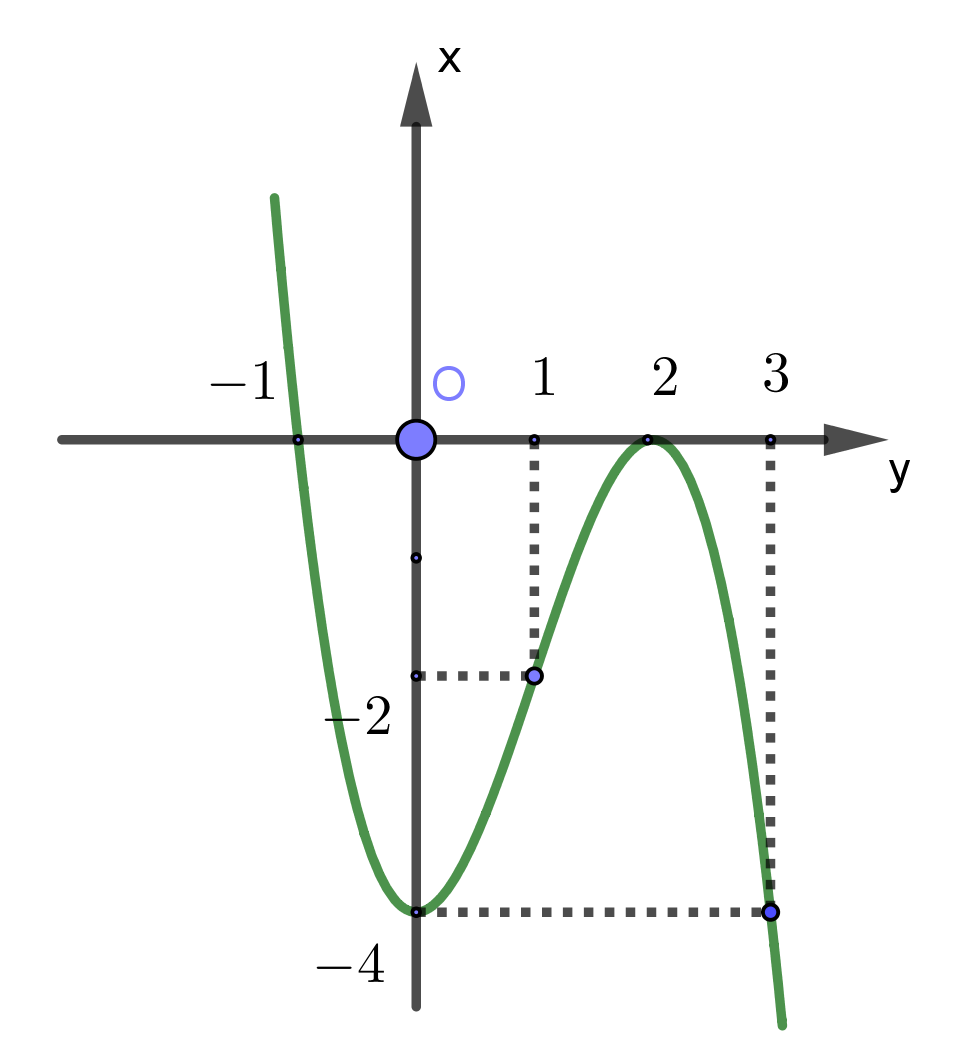
\includegraphics[width=6cm]{images/quizz2/quizz_2_figure.png}
		\caption{Hình vẽ đồ thị bài 2}
	\end{figure}
	Cho $x = 1 \Rightarrow y = 0$ \\
	Cho $x = 3 \Rightarrow y = -4$
\item Điểm uốn:
	$$y^{\prime\prime} = -6x + 6 = 0 \Leftrightarrow x = 1$$
	Khi $x = 1 \Rightarrow y(-1) = 2$ \\
	Đồ thị hàm số nhận điểm $I(-1, 2)$ làm điểm uốn. 
\end{itemize}

%\section*{Bài 3:}
Giải phương trình:
\begin{enumerate}[label=(\alph*)]
\item $(x^2 - x - 2)\sqrt{x+1} = 0$
\item $\frac{x^2}{\sqrt{x-2}}=\frac{1}{\sqrt{x-2}} - \sqrt{x-2}$
\end{enumerate}

\subsection*{Lời giải:}
\begin{enumerate}[label=(\alph*)]
\item Điều kiện xác định: $x \geq -1$ \\
Ta có $x=-1$ là một nghiệm. \\
Nếu $x > 1$ thì $\sqrt{x+1} > 0$. \\
Do đó phương trình tương  $x^2 - x -2 = 0 \Leftrightarrow x=-1$ hoặc $x=2$ \\
Đối chiếu điều kiện ta được nghiệm của phương trình là $x = -1, x = 2$. \\
Vậy phương trình đã cho có hai nghiệm S = $\{-1; 2\}$
\item Điều kiện xác định: $x > 2$ \\
 Với điệu kiện đó phương trình tương đương với phương trình:
\begin{eqnarray*}
x^2 &=& 1 - (x-2) \\
x^2 + x -3 &=& 0 \\
x &=& \frac{-1 \pm \sqrt{13}}{2}
\end{eqnarray*}
Đối chiếu với điều kiện ta thấy không có giá trị nào thỏa mãn. \\
Vậy phương trình vô nghiệm
\end{enumerate}
\section*{Bài 3:}
Giải phương trình:
\begin{enumerate}[label=(\alph*)]
\item $(x^2 - x - 2)\sqrt{x+1} = 0$
\item $\frac{x^2}{\sqrt{x-2}}=\frac{1}{\sqrt{x-2}} - \sqrt{x-2}$
\item $x + \frac{1}{x-1} = \frac{2x-1}{x-1}$
\item $1 + \frac{1}{x-3} = \frac{5}{x^2-x-6}$
\end{enumerate}

\subsection*{Lời giải:}
\begin{enumerate}[label=(\alph*)]
\item Điều kiện xác định: $x \geq -1$ \\
Ta có $x=-1$ là một nghiệm. \\
Nếu $x > 1$ thì $\sqrt{x+1} > 0$. \\
Do đó phương trình tương  $x^2 - x -2 = 0 \Leftrightarrow x=-1$ hoặc $x=2$ \\
Đối chiếu điều kiện ta được nghiệm của phương trình là $x = -1, x = 2$. \\
Vậy phương trình đã cho có hai nghiệm S = $\{-1; 2\}$

\item Điều kiện xác định: $x > 2$ \\
 Với điệu kiện đó phương trình tương đương với phương trình:
\begin{eqnarray*}
x^2 &=& 1 - (x-2) \\
x^2 + x -3 &=& 0 \\
x &=& \frac{-1 \pm \sqrt{13}}{2}
\end{eqnarray*}
Đối chiếu với điều kiện ta thấy không có giá trị nào thỏa mãn. \\
Vậy phương trình vô nghiệm

\item Điều kiện $x \neq 1$ \\
Với điều kiện trên phương trình tương đương với:\\
\begin{eqnarray*}
x^2 - x + 1 = 2x -1 \\
x = 1 \quad \textrm{or} \quad x = 2
\end{eqnarray*}
Đối chiếu điều kiện ta được phương trình có nghiệm duy nhất $x = 2$.

\item Điều kiện xác đinh:
\begin{displaymath}
\left\{ \begin{array}{l}
x \neq 3 \\
x^2 -x -6 \neq 0
\end{array} \right.  \; \Leftrightarrow \; \left\{ \begin{array}{l}
x \neq 3 \\
x \neq -2
\end{array} \right.
\end{displaymath}
Với điều kiện đó phương trình tương đương với\\
\begin{eqnarray*}
1 + \frac{1}{x-3} &=& \frac{5}{(x-3)(x+2)} \\
(x-3)(x+2) + x + 2 &=& 5 \\
x^2 &=& 9 \\
x &=& \pm 3
\end{eqnarray*}
Đối chiếu với điều kiện ta có nghiệm của phương trình là $x = -3$
\end{enumerate}
\end{document}